\chapter{संयुग्मित कार्बोनिल: माइकल और रॉबिन्सन}\label{ch:b2:conjugate-additions}

किसी स्टेरॉयड हॉर्मोन के चार वलय पहली बार एक-एक वलय करके जोड़े गए थे, और अभिक्रियाओं का एक अनुक्रम
वलय जोड़ने का मानक तरीका बन गया: यह किसी कीटोन और एक छोटे असंतृप्त कीटोन से पूरा षट्सदस्यी वलय,
कीटोन सहित, बनाता है। यह इसलिए काम करता है कि \ce{C=C} द्वि-आबंध से संयुग्मित कार्बोनिल समूह
अपना इलेक्ट्रॉनरागी गुण उस द्वि-आबंध के दूर वाले सिरे तक पहुँचा देता है।
यह अध्याय उसी दूर वाले सिरे के बारे में है: कौन-से नाभिकरागी उस पर आक्रमण करते हैं, क्यों, और उससे क्या बनाया जा सकता है।

\begin{recall}
\Cref{ch:b2:enolates-aldol}: \omterm{def:b2:enolates-aldol:enolate}{ईनोलेट}, \omterm{def:b2:enolates-aldol:aldol}{ऐल्डोल संघनन}। \Cref{ch:b2:frontier-orbitals}: आवेश
और \omterm{def:b2:frontier-orbitals:control}{कक्षक नियंत्रण}, कठोर और मृदु अभिकर्मक। \Cref{ch:b2:huckel}: ह्युकेल कक्षक और $\pi$ आवेश।
प्रथम वर्ष का खंड: ग्रीन्यार अभिकर्मक और हाइड्राइड, गतिक और ऊष्मागतिक नियंत्रण, संयुग्मित
निकाय।
\end{recall}

\section{दो इलेक्ट्रॉनरागी स्थल}

\begin{definition}[$\alpha,\beta$-असंतृप्त कार्बोनिल यौगिक]\label{def:b2:conjugate-additions:enone}
\emph{$\alpha,\beta$-असंतृप्त कार्बोनिल यौगिक}\index{अल्फ़ा,बीटा-असंतृप्त कार्बोनिल यौगिक@$\alpha,\beta$-असंतृप्त कार्बोनिल यौगिक}
में किसी कार्बोनिल यौगिक के $\alpha$
और $\beta$ कार्बनों के बीच एक \ce{C=C} द्वि-आबंध होता है, जो \ce{C=O} से संयुग्मित हो: ईनोन (कीटोन), ईनैल
(ऐल्डिहाइड), कोई असंतृप्त एस्टर या \omterm{def:b2:amines:nitrile}{नाइट्राइल}। सबसे सरल प्रोपीनल \ce{CH2=CHCHO} और
ब्यूट-3-ईन-2-ओन \ce{CH2=CHCOCH3} (मेथिल वाइनिल कीटोन) हैं।
\end{definition}

\begin{omfigure}
\setchemfig{atom sep=1.9em}
\schemestart
\chemfig{H_2C=CH-CH=O}
\arrow{<->}
\chemfig{H_2C=CH-\chemabove{C}{\scriptstyle +}H-\chemabove{O}{\scriptstyle -}}
\arrow{<->}
\chemfig{\chemabove{C}{\scriptstyle +}H_2-CH=CH-\chemabove{O}{\scriptstyle -}}
\schemestop
\par\medskip

\begin{tikzpicture}
\begin{axis}[ybar, width=0.47\linewidth, height=4.6cm, ymin=-0.6, ymax=0.4,
  xtick={1,2,3,4}, xticklabels={C$\beta$,C$\alpha$,C(O),O}, axis x line=bottom, axis y line=left,
  extra y ticks={0}, extra y tick style={grid=major, grid style={black!50}}, enlarge x limits=0.15,
  tick label style={font=\scriptsize}, ylabel={$\pi$ आवेश}, label style={font=\small},
  title={\small प्रोपीनल के $\pi$ आवेश}, bar width=8pt]
\addplot[fill=omDef!50, draw=omDef] table[x=atom, y=q] {figdata/out/bachelor-2-huckel-d.dat};
\end{axis}
\end{tikzpicture}\hfill
\begin{tikzpicture}
\begin{axis}[ybar, width=0.47\linewidth, height=4.6cm, ymin=-0.8, ymax=0.8,
  xtick={1,2,3,4}, xticklabels={C$\beta$,C$\alpha$,C(O),O}, axis x line=bottom, axis y line=left,
  extra y ticks={0}, extra y tick style={grid=major, grid style={black!50}}, enlarge x limits=0.15,
  tick label style={font=\scriptsize}, ylabel={गुणांक}, label style={font=\small},
  title={\small प्रोपीनल का LUMO}, bar width=8pt]
\addplot[fill=omThm!45, draw=omThm] table[x=atom, y=c] {figdata/out/bachelor-2-huckel-d.dat};
\end{axis}
\end{tikzpicture}

{\small प्रोपीनल। ऊपर: इसकी तीन अनुनादी संरचनाएँ; अंतिम दो कार्बोनिल कार्बन और
$\beta$ कार्बन पर धनात्मक आवेश रखती हैं। नीचे: \cref{ch:b2:frontier-orbitals} का
ह्युकेल मॉडल ($\alpha_{\ce{O}} = \alpha + \beta$, $\beta_{\ce{CO}} = \beta$; एक मॉडल)।
सबसे बड़ा धनात्मक आवेश कार्बोनिल कार्बन पर है (+0.33, जबकि $\beta$ कार्बन पर +0.23); सबसे बड़ा
\omterm{def:b2:frontier-orbitals:frontier}{LUMO} गुणांक $\beta$ कार्बन पर है (0.66, जबकि $-0.58$)।}
\end{omfigure}

\begin{proposition}[दो स्थल]\label{prop:b2:conjugate-additions:two-sites}
किसी $\alpha,\beta$-असंतृप्त कार्बोनिल यौगिक में कार्बोनिल कार्बन और $\beta$ कार्बन दोनों
इलेक्ट्रॉनरागी हैं। कार्बोनिल कार्बन बड़ा धनात्मक आवेश वहन करता है; $\beta$ कार्बन \omterm{def:b2:frontier-orbitals:frontier}{LUMO} में
बड़ा गुणांक वहन करता है।
\end{proposition}

\begin{proof}[तर्क]
अनुनादी संरचनाएँ कार्बोनिल कार्बन पर और, \ce{C=C} के माध्यम से,
$\beta$ कार्बन पर धनात्मक आवेश रखती हैं; $\alpha$ कार्बन कभी धनात्मक नहीं होता। प्रोपीनल का ह्युकेल मॉडल इसे
मात्रात्मक बनाता है: $2c^2$ का योग, दोनों भरे $\pi$ कक्षकों पर, $\pi$ आवेश देता है
(\cref{def:b2:huckel:indices}): $+0.33$ कार्बोनिल कार्बन पर, $+0.23$ $\beta$ कार्बन पर, $-0.03$
$\alpha$ कार्बन पर और $-0.53$ ऑक्सीजन पर। \omterm{def:b2:frontier-orbitals:frontier}{LUMO}, वह कक्षक जो नाभिकरागी के इलेक्ट्रॉन ग्रहण करता है,
$\beta$ कार्बन पर सबसे बड़ा है। इसलिए दोनों स्थल \cref{def:b2:frontier-orbitals:control} के दो प्रकार के
नियंत्रण के अनुरूप हैं।
% figdata: bachelor-2/huckel.py part d
\end{proof}

\section{1,2-योग या संयुग्मी योग}

\begin{definition}[योग के प्रकार]\label{def:b2:conjugate-additions:addition-modes}
किसी $\alpha,\beta$-असंतृप्त कार्बोनिल यौगिक के कार्बोनिल कार्बन से जुड़ने वाला नाभिकरागी
\emph{1,2-योग}\index{1,2-योग} देता है (ऑक्सीजन से गिनते हुए): एक ऐलिलिक ऐल्कॉक्साइड, फिर एक
ऐल्कोहॉल। $\beta$ कार्बन से जुड़ने वाला नाभिकरागी \emph{संयुग्मी योग}\index{संयुग्मी योग}
(या 1,4-योग) देता है: एक \omterm{def:b2:enolates-aldol:enolate}{ईनोलेट}, जो कार्बन पर प्रोटॉनित होकर $\beta$ कार्बन पर प्रतिस्थापित एक संतृप्त कार्बोनिल
यौगिक देता है।
\end{definition}

\begin{omfigure}
\setchemfig{atom sep=1.9em}
\schemestart
\chemfig{*6(-=-(=O)---)}
\arrow{->[\ce{CH3Li}][फिर \ce{H2O}]}[,1.4]
\chemfig{*6(-=-(-[:75]CH_3)(-[:-15]OH)---)}
\schemestop
\hspace{2.5em}
\schemestart
\chemfig{*6(-=-(=O)---)}
\arrow{->[\ce{(CH3)2CuLi}][फिर \ce{H2O}]}[,1.6]
\chemfig{*6(-(-CH_3)--(=O)---)}
\schemestop
\par\vspace{6pt}

{\small दो मेथिल नाभिकरागियों के साथ साइक्लोहेक्स-2-ईन-1-ओन। मेथिललिथियम, एक \omterm{def:b2:frontier-orbitals:hard-soft}{कठोर नाभिकरागी},
कार्बोनिल कार्बन से जुड़ता है: 1-मेथिलसाइक्लोहेक्स-2-ईन-1-ऑल (\omterm{def:b2:conjugate-additions:addition-modes}{1,2-योग})। लिथियम डाइमेथिलक्यूप्रेट, एक \omterm{def:b2:frontier-orbitals:hard-soft}{मृदु नाभिकरागी},
$\beta$ कार्बन से जुड़ता है: 3-मेथिलसाइक्लोहेक्सेनोन (\omterm{def:b2:conjugate-additions:addition-modes}{संयुग्मी योग})।}
\end{omfigure}

\begin{proposition}[कौन-सा स्थल]\label{prop:b2:conjugate-additions:regio}
\omterm{def:b2:frontier-orbitals:hard-soft}{कठोर नाभिकरागी} (कार्बलिथियम, अधिकांश ग्रीन्यार अभिकर्मक, \ce{LiAlH4}) मुख्यतः 1,2 जुड़ते हैं, \omterm{def:b2:frontier-orbitals:control}{आवेश
नियंत्रण} में, प्रायः अनुत्क्रमणीय रूप से। \omterm{def:b2:frontier-orbitals:hard-soft}{मृदु नाभिकरागी} (\omterm{def:b2:conjugate-additions:cuprate}{कार्बक्यूप्रेट}, स्थायीकृत \omterm{def:b2:enolates-aldol:enolate}{ईनोलेट}, थायोलेट,
ऐमीन) मुख्यतः 1,4 जुड़ते हैं, \omterm{def:b2:frontier-orbitals:control}{कक्षक नियंत्रण} में; संयुग्मी योगज, जो \ce{C=O} आबंध बनाए रखता है,
अधिक स्थायी उत्पाद भी है।
\end{proposition}

\begin{proof}[तर्क]
\omterm{def:b2:frontier-orbitals:hard-soft}{कठोर नाभिकरागी}, छोटा और आवेशित, मुख्यतः आवेशों के माध्यम से अन्योन्यक्रिया करता है: वह सबसे धनात्मक
केंद्र, कार्बोनिल कार्बन, पर जाता है (\cref{prop:b2:conjugate-additions:two-sites}); उसका योग तेज़ है और
उलटता नहीं, अतः 1,2-उत्पाद, जो तेज़ी से बनता है, बना रहता है (गतिक नियंत्रण)। \omterm{def:b2:frontier-orbitals:hard-soft}{मृदु नाभिकरागी},
बड़ा और ध्रुवणीय, ऊँचे \omterm{def:b2:frontier-orbitals:frontier}{HOMO} वाला, मुख्यतः \omterm{def:b2:frontier-orbitals:frontier}{अग्रांत कक्षकों} के माध्यम से अन्योन्यक्रिया करता है: वह वहाँ जाता है जहाँ
\omterm{def:b2:frontier-orbitals:frontier}{LUMO} सबसे बड़ा है, $\beta$ कार्बन। 1,4-उत्पाद एक \ce{C=O} $\pi$ आबंध बनाए रखता है, जो 1,2-उत्पाद द्वारा बनाए रखे गए
\ce{C=C} $\pi$ आबंध से प्रबल है; जब योग उत्क्रमणीय होते हैं (सायनाइड, ऐमीन,
स्थायीकृत \omterm{def:b2:enolates-aldol:enolate}{ईनोलेट}, ऐल्कॉक्साइड), तो साम्य संयुग्मी योगज की ओर खिसकता है, तब भी जब
1,2-योगज पहले बना हो (ऊष्मागतिक नियंत्रण)।
\end{proof}

\begin{method}[योग के प्रकार का पूर्वानुमान]\label{met:b2:conjugate-additions:predict-mode}
\begin{enumerate}
  \item नाभिकरागी का वर्गीकरण कीजिए: कठोर (\ce{RLi}, \ce{RMgX}, \ce{LiAlH4}, ऐल्डिहाइड के साथ \ce{NaBH4})
        या मृदु (\ce{R2CuLi}, कोई 1,3-डाइकार्बोनिल \omterm{def:b2:enolates-aldol:enolate}{ईनोलेट}, \ce{RS-}, \ce{R2NH}, साम्य पर सायनाइड)।
  \item उत्क्रमणीयता जाँचिए: अनुत्क्रमणीय कठोर योग 1,2-उत्पाद देता है; उत्क्रमणीय योग,
        समय मिलने पर, 1,4-उत्पाद।
  \item बाधा जाँचिए: प्रतिस्थापित $\beta$ कार्बन 1,4-योग को धीमा करता है; ऐल्डिहाइड, जो कीटोन से कम बाधित
        और अपने कार्बोनिल पर अधिक अभिक्रियाशील है, 1,2 के अनुकूल है।
  \item 1,4-योग से बना \omterm{def:b2:enolates-aldol:enolate}{ईनोलेट} लिखिए: उसे प्रोटॉनित किया जा सकता है, या किसी
        इलेक्ट्रॉनरागी से पकड़ा जा सकता है।
\end{enumerate}
\end{method}

\section{माइकल योग}

\begin{definition}[माइकल योग]\label{def:b2:conjugate-additions:michael}
\emph{माइकल योग}\index{माइकल योग} किसी स्थायीकृत कार्बऋणायन,
प्रायः किसी \omterm{def:b2:enolates-aldol:enolate}{ईनोलेट}, का किसी $\alpha,\beta$-असंतृप्त कार्बोनिल यौगिक या इसी प्रकार की इलेक्ट्रॉन-निर्धन
ऐल्कीन पर \omterm{def:b2:conjugate-additions:addition-modes}{संयुग्मी योग} है। नाभिकरागी \emph{माइकल दाता}\index{माइकल दाता} है (कोई 1,3-डाइकार्बोनिल यौगिक, कोई
नाइट्रोऐल्केन, कोई सायनोएस्टर); असंतृप्त यौगिक \emph{माइकल ग्राही}\index{माइकल ग्राही} है
(कोई ईनोन, कोई ईनैल, कोई असंतृप्त एस्टर, \omterm{def:b2:amines:nitrile}{नाइट्राइल} या नाइट्रो यौगिक)।
\end{definition}

\begin{omfigure}
\setchemfig{atom sep=1.8em}
\schemestart
\chemfig{CH_2(-[:30]COOEt)(-[:-30]COOEt)}
\arrow{<=>[\ce{EtO-}][$-$ \ce{EtOH}]}[,1.3]
\chemfig{\chemabove{C}{\scriptstyle -}H(-[:30]COOEt)(-[:-30]COOEt)}
\+
\chemfig{H_2C=CH-C(=[2]O)-CH_3}
\schemestop

\medskip
\setchemfig{atom sep=1.6em}
\schemestart
\arrow{->[योग]}[,0.95]
\chemfig{CH(-[:150]EtOOC)(-[:210]EtOOC)-CH_2-CH=C(-[2]\chemabove{O}{\scriptstyle -})-CH_3}
\arrow{->[\ce{EtOH}][$-$ \ce{EtO-}]}[,1.1]
\chemfig{CH(-[:150]EtOOC)(-[:210]EtOOC)-CH_2-CH_2-C(=[2]O)-CH_3}
\schemestop
\par\vspace{6pt}

{\small ब्यूट-3-ईन-2-ओन पर डाइएथिल प्रोपेनडाइओएट का \omterm{def:b2:conjugate-additions:michael}{माइकल योग}। एथॉक्साइड स्थायीकृत
\omterm{def:b2:enolates-aldol:enolate}{ईनोलेट} बनाता है; यह $\beta$ कार्बन से जुड़ता है; बना \omterm{def:b2:enolates-aldol:enolate}{ईनोलेट} एथेनॉल से एक प्रोटॉन लेता है, जिससे
एथॉक्साइड का पुनर्जनन होता है। उत्पाद, डाइएथिल (3-ऑक्सोब्यूटिल)प्रोपेनडाइओएट, एक 1,5-डाइकार्बोनिल
यौगिक है।}
\end{omfigure}

\begin{proposition}[माइकल क्रियाविधि]\label{prop:b2:conjugate-additions:michael}
\omterm{def:b2:conjugate-additions:michael}{माइकल योग} तीन चरणों में चलता है (दाता का विप्रोटॉनन, \omterm{def:b2:conjugate-additions:addition-modes}{संयुग्मी योग}, नए \omterm{def:b2:enolates-aldol:enolate}{ईनोलेट} का
प्रोटॉनन), और अंतिम चरण में क्षारक का पुनर्जनन होता है: उत्प्रेरकी मात्रा पर्याप्त है।
\end{proposition}

\begin{proof}[तर्क]
दो कार्बोनिलों के बीच स्थित दाता का $\alpha$ हाइड्रोजन अम्लीय है: डाइएथिल प्रोपेनडाइओएट के लिए $\mathrm pK_a$ लगभग 13,
एथिल 3-ऑक्सोब्यूटेनोएट के लिए 10.7। एथॉक्साइड (एथेनॉल, 15.9) इसे बड़े अंश तक हटाता है, जो
पर्याप्त से अधिक है। स्थायीकृत, मृदु \omterm{def:b2:enolates-aldol:enolate}{ईनोलेट} 1,4 जुड़ता है
(\cref{prop:b2:conjugate-additions:regio})। बना \omterm{def:b2:enolates-aldol:enolate}{ईनोलेट} दाता के \omterm{def:b2:enolates-aldol:enolate}{ईनोलेट} से प्रबल क्षारक है
(वह एक कार्बोनिल से स्थायीकृत है, दो से नहीं), अतः वह विलायक से एक प्रोटॉन लेता है, और
उपभुक्त एथॉक्साइड के बदले एक एथॉक्साइड लौटा देता है। समग्र अभिक्रिया एक \ce{C-C} $\sigma$ आबंध बनाती है,
एक \ce{C=C} $\pi$ आबंध से: यह अनुकूल है, और स्थायीकृत दाता के साथ योगज वापस नहीं लौटता।
% ledger: pka:ethanol, pka:diethylmalonate, pka:acetoacetate
\end{proof}

दाता की ओर एक कीटोन और ग्राही की ओर एक कीटोन वाला माइकल योगज एक 1,5-डाइकार्बोनिल
यौगिक है: दोनों कार्बोनिल पाँच कार्बन दूर हैं, दोनों कार्बोनिल कार्बनों को गिनते हुए। यही पैटर्न
\omterm{def:b2:conjugate-additions:michael}{माइकल योग} का चिह्न है, जैसे $\beta$-हाइड्रॉक्सी कार्बोनिल \omterm{def:b2:enolates-aldol:aldol}{ऐल्डोल} का था
(\cref{met:b2:enolates-aldol:aldol-recognition})।

\section{कार्बक्यूप्रेट}

\begin{definition}[कार्बक्यूप्रेट]\label{def:b2:conjugate-additions:cuprate}
\emph{कार्बक्यूप्रेट}\index{कार्बक्यूप्रेट} \ce{R2CuLi} दो कार्बनिक समूह धारण करने वाला एक कॉपर(I) यौगिक है,
जो किसी कार्बलिथियम के दो तुल्यांकों और किसी कॉपर(I) हैलाइड के एक तुल्यांक से बनता है:
\begin{equation*}
\ce{2 CH3Li + CuI -> (CH3)2CuLi + LiI}.
\end{equation*}
\end{definition}

\omterm{def:b2:conjugate-additions:cuprate}{कार्बक्यूप्रेट} (जिन्हें गिलमैन अभिकर्मक भी कहते हैं) अपने जनक कार्बलिथियमों की तरह निम्न ताप पर,
अक्रिय गैस के अंतर्गत, ईथर में बनाए और प्रयुक्त किए जाते हैं। कॉपर लिथियम या
मैग्नीशियम से कम विद्युत-धनात्मक है, अतः \ce{Cu-C} आबंध अधिक सहसंयोजी है और कार्बन कम आवेशित: किसी
क्यूप्रेट का मेथिल समूह \omterm{def:b2:frontier-orbitals:hard-soft}{मृदु नाभिकरागी} है। इसके तीन उपयोग हैं।

\begin{itemize}
  \item किसी ईनोन पर ऐल्किल या ऐरिल समूह का \emph{\omterm{def:b2:conjugate-additions:addition-modes}{संयुग्मी योग}}, जो ग्रीन्यार अभिकर्मक और
        कार्बलिथियम स्वच्छ रूप से नहीं करते; दोनों \ce{R} समूहों में से केवल एक स्थानांतरित होता है।
  \item \emph{पकड़ना}: \omterm{def:b2:conjugate-additions:addition-modes}{संयुग्मी योग} से बने \omterm{def:b2:enolates-aldol:enolate}{ईनोलेट} का उसके $\alpha$
        कार्बन पर ऐल्किलन किया जा सकता है, जिससे एक ही संक्रिया में दो नए \ce{C-C} आबंध बनते हैं।
  \item हैलाइडों का \emph{प्रतिस्थापन}: $\mathrm{R_2CuLi + R'Br \to R{-}R' + RCu + LiBr}$, एक ऐसा युग्मन जिसे
        कोई कार्बलिथियम विलोपन या विनिमय करके बिगाड़ देता।
\end{itemize}

\section{रॉबिन्सन वलयन}

\begin{definition}[वलयन]\label{def:b2:conjugate-additions:robinson}
\emph{वलयन}\index{वलयन} किसी विद्यमान अणु पर एक नया वलय बनाता है। \emph{रॉबिन्सन वलयन}
\index{रॉबिन्सन वलयन} एक साइक्लोहेक्स-2-ईन-1-ओन बनाता है: किसी कीटोन के
\omterm{def:b2:enolates-aldol:enolate}{ईनोलेट} का किसी $\alpha,\beta$-असंतृप्त कीटोन (प्रायः ब्यूट-3-ईन-2-ओन) पर \omterm{def:b2:conjugate-additions:michael}{माइकल योग}, और उसके बाद
बने 1,5-डाइकीटोन का अंतःअणुक \omterm{def:b2:enolates-aldol:aldol}{ऐल्डोल संघनन}।
\end{definition}

\begin{omfigure}
\setchemfig{atom sep=1.8em}
\schemestart
\chemfig{[:30]*6(-(=O)-(-CH_3)-(=O)---)}
\+
\chemfig{=[:30]-[:-30](=[:-90]O)-[:30]}
\arrow{->[क्षारक][माइकल]}[,1.2]
\chemfig{[:30]*6(-(=O)-(-[:40]CH_3)(-[:-30]-[:30]-[:-30](=[:-90]O)-[:30])-(=O)---)}
\schemestop

\medskip
\schemestart
\arrow{->[क्षारक][ऐल्डोल]}[,1.1]
\chemfig{[:-30]*6(---(-[:-60]OH)*6(--(=O)---)-(-[:105]CH_3)-(=O)-)}
\arrow{->[ताप][$-$ \ce{H2O}]}[,1.1]
\chemfig{[:-30]*6(---*6(=-(=O)---)-(-[:105]CH_3)-(=O)-)}
\schemestop
\par\vspace{6pt}

{\small वह \omterm{def:b2:conjugate-additions:robinson}{रॉबिन्सन वलयन} जो वीलैंड--मीशर कीटोन बनाता है।
2-मेथिलसाइक्लोहेक्सेन-1,3-डाइओन का \omterm{def:b2:enolates-aldol:enolate}{ईनोलेट} ब्यूट-3-ईन-2-ओन से जुड़ता है (माइकल): एक ट्राइकीटोन।
पार्श्व-शृंखला के मेथिल कीटोन का \omterm{def:b2:enolates-aldol:enolate}{ईनोलेट} वलय के एक कार्बोनिल पर आक्रमण करता है (अंतःअणुक \omterm{def:b2:enolates-aldol:aldol}{ऐल्डोल}), जिससे एक षट्सदस्यी वलय बंद होता है;
निर्जलीकरण संयुग्मित ईनोन देता है। कोणीय मेथिल समूह दोनों वलयों द्वारा साझा कार्बन पर है,
जो एकमात्र त्रिविमजनक केंद्र है।}
\end{omfigure}

\begin{proposition}[रॉबिन्सन वलयन]\label{prop:b2:conjugate-additions:robinson}
$\alpha$ हाइड्रोजन वाला कोई कीटोन और ब्यूट-3-ईन-2-ओन, क्षारक में, तीन
चरणों में एक साइक्लोहेक्स-2-ईन-1-ओन देते हैं: \omterm{def:b2:conjugate-additions:michael}{माइकल योग}, षट्सदस्यी वलय बनाने वाला अंतःअणुक \omterm{def:b2:enolates-aldol:aldol}{ऐल्डोल योग}, और निर्जलीकरण।
नए वलय में कीटोन का भूतपूर्व $\alpha$ कार्बन और उसका कार्बोनिल कार्बन, और ब्यूट-3-ईन-2-ओन के चारों
कार्बन होते हैं।
\end{proposition}

\begin{proof}
चित्र में परमाणुओं का अनुसरण कीजिए। कीटोन का \omterm{def:b2:enolates-aldol:enolate}{ईनोलेट} कार्बन (इसे C$_a$ कहिए) ब्यूट-3-ईन-2-ओन के $\beta$
कार्बन से आबंधित होता है: शृंखला C$_a$--\ce{CH2}--\ce{CH2}--\ce{C(=O)}--\ce{CH3} C$_a$ पर लटकती है, और
C$_a$ अभी भी कीटोन के कार्बोनिल कार्बन C$_k$ से आबंधित है। क्षारक में शृंखला का मेथिल कीटोन
अंतस्थ \ce{CH3} पर अपना \omterm{def:b2:enolates-aldol:enolate}{ईनोलेट} बनाता है, जो C$_k$ पर आक्रमण करता है। बंद हुए वलय में C$_k$, C$_a$,
दोनों \ce{CH2}, पार्श्व-शृंखला का कार्बोनिल कार्बन और भूतपूर्व मेथिल कार्बन गिने जाते हैं: छह परमाणु, तनाव-मुक्त
वलय आकार, यही कारण है कि संभावित ईनोलेटों में से यही \omterm{def:b2:enolates-aldol:enolate}{ईनोलेट} स्थायी उत्पाद तक ले जाता है (शृंखला के
भीतरी \ce{CH2} \omterm{def:b2:enolates-aldol:enolate}{ईनोलेट} का आक्रमण एक चतुःसदस्यी वलय बंद करता)। \omterm{def:b2:enolates-aldol:aldol}{ऐल्डोल} का
\ce{OH} C$_k$ पर है, शृंखला कार्बोनिल के सापेक्ष $\beta$; निर्जलीकरण \ce{C=C} को C$_k$ और
भूतपूर्व मेथिल कार्बन के बीच रखता है, कार्बोनिल से संयुग्मित: एक साइक्लोहेक्स-2-ईन-1-ओन।
\end{proof}

\begin{method}[किसी साइक्लोहेक्सीनोन का विच्छेदन]\label{met:b2:conjugate-additions:robinson-disconnection}
\begin{enumerate}
  \item लक्ष्य में एक साइक्लोहेक्स-2-ईन-1-ओन खोजिए; उसके कार्बोनिल कार्बन को C1, द्वि-आबंध को
        C2=C3, और वलय को C6 तक क्रमांकित कीजिए।
  \item निर्जलीकरण को उलटिए: C3 पर एक \ce{OH}, C2 पर एक \ce{C-H}।
  \item \omterm{def:b2:enolates-aldol:aldol}{ऐल्डोल} को उलटिए: C2--C3 काटिए। C3 एक कीटोन कार्बोनिल बन जाता है, C2 किसी मेथिल कीटोन का
        मेथिल समूह: एक 1,5-डाइकीटोन।
  \item \omterm{def:b2:conjugate-additions:michael}{माइकल योग} को उलटिए: C4 (C3 कीटोन का $\alpha$ कार्बन) और
        C5 के बीच का आबंध काटिए। दाता वह कीटोन है; ग्राही ईनोन C5=C6--C1(=O)--C2 है, जो
        ब्यूट-3-ईन-2-ओन है जब C5, C6 और C2 पर केवल हाइड्रोजन हों।
\end{enumerate}
\end{method}

\begin{history}[वलयन, 1935]
\begin{minipage}[t]{0.18\linewidth}
\vspace{0pt}
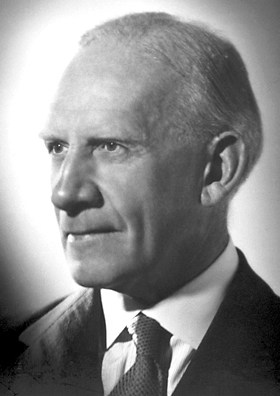
\includegraphics[width=\linewidth]{images/book3/robinson.jpg}
\end{minipage}\hfill
\begin{minipage}[t]{0.78\linewidth}
\vspace{0pt}
रॉबर्ट रॉबिन्सन और विलियम रैप्सन ने 1935 में स्टेरॉयडों के संश्लेषण को लक्ष्य बनाकर किए गए काम में
यह वलय-निर्माणकारी अनुक्रम प्रकाशित किया। रॉबिन्सन की मुख्य उपलब्धियाँ ऐल्केलॉइडों की संरचनाएँ और संश्लेषण थीं,
जिनके लिए उन्हें 1947 का रसायन का नोबेल पुरस्कार मिला। 1950 में पीटर वीलैंड और कार्ल मीशर ने
इस अध्याय की समस्या का द्विचक्रीय डाइकीटोन बनाया, जो स्टेरॉयड और
टर्पीन संश्लेषणों का एक सामान्य आरंभ-बिंदु बन गया। (चित्र: अज्ञात लेखक, सार्वजनिक अधिकार-क्षेत्र; विकिमीडिया कॉमन्स।)
\end{minipage}
\end{history}

\begin{safety}{\ghs[5mm]{GHS02}\,\ghs[5mm]{GHS05}\,\ghs[5mm]{GHS06}\,\ghs[5mm]{GHS07}\,\ghs[5mm]{GHS08}\,\ghs[5mm]{GHS09}}
ब्यूट-3-ईन-2-ओन ज्वलनशील, अत्यंत विषैला, संक्षारक और जलीय पर्यावरण के लिए हानिकारक है, और एक प्रबल अश्रुकारी; इसे केवल
धूम-हुड में सँभाला जाता है। साइक्लोहेक्स-2-ईन-1-ओन ज्वलनशील और विषैला है। कार्बलिथियम, ग्रीन्यार अभिकर्मक और
क्यूप्रेट जल से प्रचंड अभिक्रिया करते हैं और अक्रिय गैस के अंतर्गत सँभाले जाते हैं।
% ledger: ghs:MVK, ghs:cyclohexenone, ghs:MeMgBr
\end{safety}

\section{अभ्यास}

\begin{exercise}[$\star$]\label{exo:b2:conjugate-additions:1}
साइक्लोहेक्स-2-ईन-1-ओन पर 1,2- या 1,4-योग का पूर्वानुमान कीजिए, इनके लिए: \ce{CH3MgBr}; \ce{(CH3)2CuLi};
थोड़े क्षारक के साथ \ce{C6H5SH}; \ce{LiAlH4}।
\end{exercise}

\begin{exercise}[$\star$]\label{exo:b2:conjugate-additions:2}
\omterm{def:b2:conjugate-additions:michael}{माइकल दाता} या \omterm{def:b2:conjugate-additions:michael}{माइकल ग्राही} के रूप में वर्गीकृत कीजिए: पेंटेन-2,4-डाइओन, प्रोपीननाइट्राइल \ce{CH2=CHCN},
नाइट्रोमेथेन, मेथिल प्रोपीनोएट, डाइएथिल प्रोपेनडाइओएट, ब्यूट-3-ईन-2-ओन।
\end{exercise}

\begin{exercise}[$\star$]\label{exo:b2:conjugate-additions:3}
1-ब्रोमोब्यूटेन, लिथियम और कॉपर(I) आयोडाइड से लिथियम डाइब्यूटिलक्यूप्रेट का निर्माण लिखिए।
\end{exercise}

\begin{exercise}[$\star$]\label{exo:b2:conjugate-additions:4}
ब्यूट-3-ईन-2-ओन और सोडियम एथॉक्साइड की उत्प्रेरकी मात्रा के साथ डाइएथिल प्रोपेनडाइओएट का उत्पाद दीजिए,
फिर जल-अपघटन और गर्म करने के बाद का उत्पाद।
\end{exercise}

\begin{exercise}[$\star\star$]\label{exo:b2:conjugate-additions:5}
साइक्लोहेक्स-2-ईन-1-ओन से 3-मेथिलसाइक्लोहेक्सेनोन बनाने की एक विधि प्रस्तावित कीजिए, और समझाइए कि
मेथिलमैग्नीशियम ब्रोमाइड एक ख़राब विकल्प क्यों होगा।
\end{exercise}

\begin{exercise}[$\star\star$]\label{exo:b2:conjugate-additions:6}
ट्राइएथिलऐमीन के अंश के साथ एथेनथायोल ब्यूट-3-ईन-2-ओन से जुड़ता है। क्रियाविधि लिखिए और बताइए कि
थायोलेट 1,4 क्यों जुड़ता है।
\end{exercise}

\begin{exercise}[$\star\star$]\label{exo:b2:conjugate-additions:7}
निम्न ताप और कम समय पर साइक्लोहेक्स-2-ईन-1-ओन के साथ सायनाइड सायनोहाइड्रिन देता है; उच्चतर
ताप और अधिक समय पर 3-ऑक्सोसाइक्लोहेक्सेन-1-कार्बोनाइट्राइल। गतिक और ऊष्मागतिक
नियंत्रण से समझाइए।
\end{exercise}

\begin{exercise}[$\star\star$]\label{exo:b2:conjugate-additions:8}
ब्यूट-3-ईन-2-ओन के साथ 2-मेथिलसाइक्लोहेक्सेन-1,3-डाइओन का \omterm{def:b2:conjugate-additions:robinson}{रॉबिन्सन वलयन} उत्पाद दीजिए, फिर
ब्यूट-3-ईन-2-ओन के साथ साइक्लोहेक्सेनोन का।
\end{exercise}

\begin{exercise}[$\star\star$]\label{exo:b2:conjugate-additions:9}
हेप्टेन-2,6-डाइओन का एक \omterm{def:b2:conjugate-additions:michael}{माइकल दाता} और एक \omterm{def:b2:conjugate-additions:michael}{माइकल ग्राही} में विच्छेदन कीजिए, और परिस्थितियाँ प्रस्तावित कीजिए।
\end{exercise}

\begin{exercise}[$\star\star\star$]\label{exo:b2:conjugate-additions:10}
सरल \omterm{def:b2:enolates-aldol:aldol}{ऐल्डोल योग} क्षारक में आसानी से उलट जाता है; डाइएथिल प्रोपेनडाइओएट और
ब्यूट-3-ईन-2-ओन का माइकल योगज नहीं। बने और टूटे आबंधों से और उत्पाद की अम्लता से समझाइए।
\end{exercise}

\begin{exercise}[$\star\star\star$]\label{exo:b2:conjugate-additions:11}
मेथिल प्रोपीनोएट के दो तुल्यांकों और उत्प्रेरकी क्षारक के साथ डाइएथिल प्रोपेनडाइओएट ऐसा उत्पाद देता है
जिसके दोनों एस्टर समूहों के बीच कोई \ce{C-H} शेष नहीं रहता। उसे खींचिए और समझाइए।
\end{exercise}

\begin{exercise}[$\star\star\star$]\label{exo:b2:conjugate-additions:12}
\omterm{def:b2:conjugate-additions:robinson}{रॉबिन्सन वलयन} में 2-मेथिलसाइक्लोहेक्सेनोन और ब्यूट-3-ईन-2-ओन किसी भी \omterm{def:b2:enolates-aldol:enolate}{ईनोलेट} से होकर अभिक्रिया कर सकते हैं।
दोनों उत्पाद खींचिए और बताइए कि कौन-सी परिस्थितियाँ उस उत्पाद के अनुकूल हैं जिसमें मेथिल समूह वलय-संगलन
कार्बन पर है।
\end{exercise}

\section{समस्या: वीलैंड--मीशर कीटोन}

\begin{problem}[{सप्ताहांत समस्या --- अम्लीय दाता, माइकल योगज, अंतःअणुक ऐल्डोल और
उसका निर्जलीकरण, त्रिविमजनक केंद्र और एक निर्माण का द्रव्यमान संतुलन}]
\label{pb:b2:conjugate-additions:1}
निर्माण (अभ्यास के आँकड़े): 2-मेथिलसाइक्लोहेक्सेन-1,3-डाइओन के \qty{10.0}{g} ब्यूट-3-ईन-2-ओन के हल्के आधिक्य
और उत्प्रेरकी क्षारक से अभिक्रिया करते हैं (\omterm{def:b2:conjugate-additions:michael}{माइकल योग}); फिर ट्राइकीटोन का एक
\omterm{def:b2:amines:class}{द्वितीयक ऐमीन} और एक अम्ल के साथ चक्रीकरण किया जाता है (\omterm{def:b2:enolates-aldol:aldol}{ऐल्डोल}, निर्जलीकरण)। समग्र लब्धि: 70~\%। जनक साइक्लोहेक्सेन-1,3-डाइओन
का जल में $\mathrm pK_a = 5.3$ है। मोलर द्रव्यमान (\unit{g/mol}): C 12.011, H 1.008, O 15.999।
% ledger: pka:cyclohexanedione, aw:C, aw:H, aw:O, ghs:methylcyclohexanedione, ghs:MVK

\medskip
\noindent\textbf{भाग I --- दाता।}
\begin{enumerate}
  \item 2-मेथिलसाइक्लोहेक्सेन-1,3-डाइओन खींचिए और उसका सबसे अम्लीय हाइड्रोजन चिह्नित कीजिए।
  \item वह हाइड्रोजन साइक्लोहेक्सेनोन के $\alpha$ हाइड्रोजनों से इतना अधिक अम्लीय क्यों है?
  \item इसके \omterm{def:b2:enolates-aldol:enolate}{ईनोलेट} की तीन अनुनादी संरचनाएँ खींचिए।
  \item क्या हाइड्रॉक्साइड या एथॉक्साइड इस \omterm{def:b2:enolates-aldol:enolate}{ईनोलेट} को पूर्णतः बनाने के लिए पर्याप्त प्रबल है? $\mathrm pK_a$ का उपयोग कीजिए।
  \item डाइओन का वह \omterm{def:b2:enolates-aldol:tautomerism}{ईनॉल} लिखिए जिसमें C2 सम्मिलित है, और बताइए कि C2 पर मेथिल समूह
        उसे क्यों नहीं रोकता।
  \item यह \omterm{def:b2:enolates-aldol:enolate}{ईनोलेट} कठोर है या मृदु? यह ब्यूट-3-ईन-2-ओन के किस स्थल पर आक्रमण करेगा?
\end{enumerate}

\medskip
\noindent\textbf{भाग II --- माइकल योगज।}
\begin{enumerate}[resume]
  \item \omterm{def:b2:conjugate-additions:michael}{माइकल योग} लिखिए और बने ट्राइकीटोन का नाम दीजिए।
  \item क्षारक की केवल उत्प्रेरकी मात्रा क्यों चाहिए?
  \item नया आबंध डाइओन के ऑक्सीजन के बजाय उसके C2 पर क्यों बनता है?
  \item ट्राइकीटोन में कितने चतुष्क कार्बन हैं?
  \item ट्राइकीटोन में 1,5-डाइकार्बोनिल संबंध पहचानिए।
  \item ब्यूट-3-ईन-2-ओन का हल्का आधिक्य क्यों प्रयुक्त होता है, और केवल हल्का ही क्यों?
\end{enumerate}

\medskip
\noindent\textbf{भाग III --- वलय का बंद होना।}
\begin{enumerate}[resume]
  \item ट्राइकीटोन के वे कार्बन सूचीबद्ध कीजिए जिन पर $\alpha$ हाइड्रोजन हैं।
  \item कौन-सा \omterm{def:b2:enolates-aldol:enolate}{ईनोलेट}, किस कार्बोनिल पर आक्रमण करके, षट्सदस्यी वलय बंद करता है?
  \item और कौन-से वलय-बंधन आज़माए जा सकते हैं, और वे उत्पाद क्यों नहीं देते?
  \item बना \omterm{def:b2:enolates-aldol:aldol}{ऐल्डोल} और उसके बाद होने वाला निर्जलीकरण लिखिए।
  \item निर्जलीकरण आसान क्यों है?
  \item वीलैंड--मीशर कीटोन के क्रियात्मक समूहों के नाम बताइए।
\end{enumerate}

\medskip
\noindent\textbf{भाग IV --- त्रिविम-रसायन और द्रव्यमान संतुलन।}
\begin{enumerate}[resume]
  \item उत्पाद का कौन-सा कार्बन त्रिविमजनक केंद्र है?
  \item क्या इस निर्माण का उत्पाद प्रकाशिक सक्रिय है? समझाइए।
  \item डाइओन, ब्यूट-3-ईन-2-ओन और उत्पाद
        \ce{C11H14O2} के मोलर द्रव्यमान परिकलित कीजिए।
  \item समग्र समीकरण लिखिए और सूत्रों से उसकी जाँच कीजिए।
  \item प्रयुक्त डाइओन की मात्रा परिकलित कीजिए।
  \item 70~\% समग्र लब्धि पर प्राप्त वीलैंड--मीशर कीटोन का द्रव्यमान बताइए।
\end{enumerate}
\end{problem}
